\documentclass[conference,a4paper]{IEEEtran}
\usepackage[utf8]{inputenc}
\usepackage{amsmath,amssymb}
\usepackage{booktabs}
\usepackage{graphicx}
\usepackage{tikz}
\usetikzlibrary{positioning,arrows.meta}
\usepackage{xcolor}
\usepackage{url}
\usepackage[hidelinks]{hyperref}

\newcommand{\cmark}{\checkmark}

\begin{document}

\title{QuickPic: Open-Set Face Recognition for\\Classroom Attendance from a Single Group Photograph}

\author{
\IEEEauthorblockN{Tanish Mittal (20233288), Shashank Kanaujiya (20233259),\\
Utkarsh Raj Singh (20233298), Shinde Ritesh Tirupati (20233350)}
\IEEEauthorblockA{Image Processing and Computer Vision, Semester VII, Section D, Team 25\\
Motilal Nehru National Institute of Technology Allahabad, Prayagraj, India}
}

\maketitle

\begin{abstract}
Taking attendance from one photograph of a classroom is difficult. A typical photo contains dozens of faces that are small, turned away and unevenly lit, and most people in the room are not enrolled in the system at all. We present QuickPic, a pipeline that detects every face in a single class photo, recognises the enrolled students and marks every other face as unknown instead of forcing a match. The detector and the face-embedding network are pretrained and frozen. Our contribution is a classroom-aware decision layer on top of them with four switchable parts: tiled detection for small faces, degradation-aware enrollment, quality-aware score calibration, and a photo-level one-to-one assignment solved with the Hungarian method. We evaluate each part on public benchmarks (LFW, TinyFace and an Indian classroom sample from ICFD) and on ten real photographs of our own class with 804 hand-labelled faces. Tiling raises detection recall from 0.879 to 0.974. With 15 enrolled students, the deployed pipeline names 115 of 117 student appearances correctly, produces attendance lists with F1 0.966, and cuts the number of non-enrolled faces given an enrolled student's name from 32 to 6. Calibration helps for faces below 20 pixels but not at classroom face sizes. A web application (Django API, React frontend) lets students register their face with guided, automatically checked photos and lets teachers review and confirm the list.
\end{abstract}

\begin{IEEEkeywords}
face detection, open-set face recognition, low-resolution faces, score calibration, assignment problem, attendance systems
\end{IEEEkeywords}

% ---------------------------------------------------------------------------
\section{Introduction}

Roll call takes several minutes of every lecture, and sign-in sheets invite proxy attendance. Face recognition is a natural replacement, but most attendance systems assume one person at a time in front of a camera. We study a harder and more practical setting: the teacher takes one photograph of the whole room, and the system produces a draft attendance list that the teacher confirms or corrects.

Three properties of classroom photos make this a computer vision problem rather than a database lookup. First, faces at the back of the room may be only 20 to 40 pixels tall, below the scale at which detectors and recognisers are usually evaluated. Second, students look in different directions and sit under uneven lighting. Third, the task is \emph{open-set}, meaning the system must also recognise when a face belongs to nobody it knows: in our class of 70 to 90 students only a minority are enrolled, so most detected faces must be rejected as unknown. A system that always returns its nearest enrolled student marks absent students present, which is the error that matters most for attendance.

\textbf{Background.} Viola and Jones~\cite{viola} made real-time face detection practical with Haar-like features and a boosted cascade. WIDER FACE~\cite{wider} showed how far such detectors fall short on small and turned faces. Modern detectors such as SCRFD~\cite{scrfd} and the tiny CPU detector YuNet~\cite{yunet} predict boxes and five landmarks directly, and slicing an image into overlapping tiles improves recall on small objects without retraining~\cite{sahi}. Classical recognisers describe a face with local binary pattern (LBP) histograms~\cite{lbp}; deep recognisers learn an embedding in which faces of one person lie close together, most commonly with the ArcFace angular-margin loss~\cite{arcface}, with lightweight variants such as SFace~\cite{sface} and MobileFaceNets~\cite{mbf}. Accuracy drops sharply at low resolution; TinyFace~\cite{tinyface} provides natively tiny faces (about $20\times16$ pixels) with a 1:N protocol, and MagFace~\cite{magface} shows that a face-quality estimate can be folded into the comparison. Open-set recognition~\cite{scheirer} formalises the need to reject unseen identities.

Closest to our setting, Bhattacharjee and Das~\cite{icfd} collected the Indian Classroom Face Dataset (ICFD) at IIT Madras and trained a generative network to enhance low-resolution classroom faces. Mery \emph{et al.}~\cite{mery} built an attendance system for crowded classrooms from smartphone photos, but evaluated it closed-set. We instead keep both networks frozen and adapt only the decision layer, and we evaluate open-set, counting how often a stranger is given an enrolled student's name.

Our contributions are: (i) an end-to-end CPU pipeline from one class photo to an editable attendance list; (ii) a decision layer with four separately switchable components placed on frozen pretrained networks; (iii) an ablation of each component on public benchmarks and on real class photos, reported with attendance-level metrics; and (iv) a working web system for enrollment, review and confirmation.

% ---------------------------------------------------------------------------
\section{Methodology}

Fig.~\ref{fig:pipeline} shows the pipeline. In plain terms: find every face, straighten it, turn it into a list of 512 numbers (an \emph{embedding}) such that photos of the same person give similar numbers, compare it with each enrolled student, and decide names for the whole photo at once. Every stage sits behind a common interface, so each comparison and \emph{ablation} (switching one component off to measure what it adds) is a configuration change.

\begin{figure}[t]
\centering
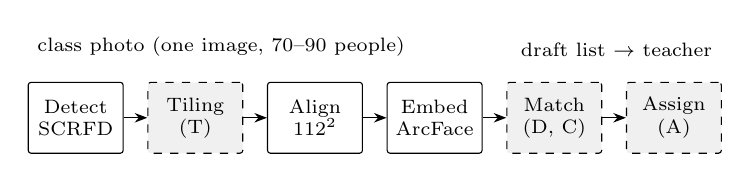
\begin{tikzpicture}[
  node distance=3mm,
  every node/.style={font=\scriptsize, align=center},
  frozen/.style={draw, rounded corners=1pt, minimum height=9mm, text width=11mm, inner sep=1.5pt},
  ours/.style={frozen, dashed, fill=gray!12},
  arr/.style={-{Stealth[length=1.6mm]}}
]
\node[frozen] (det) {Detect\\SCRFD};
\node[ours, right=of det] (tile) {Tiling\\(T)};
\node[frozen, right=of tile] (al) {Align\\$112^2$};
\node[frozen, right=of al] (emb) {Embed\\ArcFace};
\node[ours, right=of emb] (match) {Match\\(D, C)};
\node[ours, right=of match] (asg) {Assign\\(A)};
\draw[arr] (det) -- (tile); \draw[arr] (tile) -- (al); \draw[arr] (al) -- (emb);
\draw[arr] (emb) -- (match); \draw[arr] (match) -- (asg);
\node[above=2mm of det.north west, anchor=south west] {class photo (one image, 70--90 people)};
\node[above=2mm of asg.north east, anchor=south east] {draft list $\rightarrow$ teacher};
\end{tikzpicture}
\caption{The QuickPic pipeline. Solid boxes: pretrained, frozen networks. Shaded dashed boxes: the classroom-aware decision layer we contribute.}
\label{fig:pipeline}
\end{figure}

\subsection{Detection, alignment and embedding}
A detector returns a box and five landmarks (eyes, nose tip, mouth corners) for each face. We compare a Haar cascade~\cite{viola} (with CLAHE contrast enhancement), YuNet~\cite{yunet} and SCRFD~\cite{scrfd} at 10\,GF and 500\,MF. Each face is aligned by the least-squares similarity transform that maps its landmarks onto the standard ArcFace template, giving a $112\times112$ crop. A frozen network $\phi$ maps the crop to an L2-normalised embedding $f_i=\phi(x_i)$; we compare ArcFace ResNet-50 and MobileFaceNet~\cite{arcface,mbf} (InsightFace, trained on WebFace~\cite{webface}), SFace~\cite{sface} and, as a classical baseline, a $7\times7$ grid of uniform LBP histograms~\cite{lbp}.

\subsection{Baseline matching}
Student $j$ is enrolled with a gallery $G_j$ of embeddings. The baseline scores face $i$ against student $j$ by the best cosine similarity,
\begin{equation}
S_{ij} = \max_{g \in G_j} f_i^{\top} g ,
\label{eq:score}
\end{equation}
assigns each face to its best-scoring student if that score exceeds a global threshold $\tau$, and marks it unknown otherwise.

\subsection{Tiled detection (T)}
Detectors resize the whole photo to a fixed input such as $640\times640$. In a 4032-pixel phone photo a 40-pixel face shrinks to about 6 pixels and is lost. We run the detector on overlapping $1280\times1280$ tiles (25\% overlap) at native resolution plus one pass over the full image, drop boxes cut by an inner tile edge, and merge the rest with non-maximum suppression at IoU 0.4.

\subsection{Degradation-aware enrollment (D)}
Enrollment photos are sharp and close-up, while classroom faces are small, blurred and badly lit. We enlarge each gallery with synthetic copies $T_k(x)$ of every enrollment photo $x\in E_j$: downscaling to 16--48 pixels and back, Gaussian blur, gamma shifts, JPEG compression and horizontal flips ($K=10$),
\begin{equation}
G_j = \{\, \phi(T_k(x)) : x \in E_j,\ k=0,\dots,K \,\}.
\end{equation}

\subsection{Quality-aware calibration (C)}
A correct match scores lower when the face is small or blurred, and unrelated low-quality faces also look more alike, so one threshold is too strict for some faces and too lenient for others. A logistic regression turns the raw score into a match probability conditioned on face height $h_i$ and sharpness $b_i$ (variance of the Laplacian~\cite{laplacian}):
\begin{multline}
P_{ij} = \sigma\big(w_0 + w_1 S_{ij} + w_2 \log h_i \\
+ w_3 \log(1{+}b_i) + w_4 S_{ij}\log h_i\big).
\end{multline}
It is fitted on 46,494 genuine and impostor pairs from LFW~\cite{lfw}, with the probe photo degraded to a random height of 12--112 pixels, and people split 70/30 so it is tested on unseen identities. No class photo influences it.

\subsection{Photo-level one-to-one assignment (A)}
A student appears at most once in a photo, yet independent decisions can give two faces the same name. We decide all $F$ faces of a photo jointly against the $N$ students of the course:
\begin{equation}
\max_{z\in\{0,1\}^{F\times N}} \sum_{i,j} z_{ij}(P_{ij}-\tau)\ \ \text{s.t.}\ \sum_j z_{ij}\le1,\ \sum_i z_{ij}\le1 .
\end{equation}
Padding the matrix with one zero-valued ``unknown'' column per face makes this a square assignment problem, solved exactly by the Hungarian method~\cite{kuhn}. A pair below $\tau$ has negative value and is never chosen, so open-set rejection is kept. Without C, $P_{ij}$ is the raw score $S_{ij}$.

\subsection{Flagging uncertain names}
Some mistakes cannot be removed by any threshold: a stranger who resembles an enrolled student scores as high as some genuine matches. The decisive signal is the \emph{margin} $m_i = S_{i(1)} - S_{i(2)}$ between a face's best and second-best student. When $m_i < 0.06$, the proposed name is shown in amber with a question mark, and the teacher confirms or corrects it.

\subsection{Data and evaluation protocol}
\textbf{Public data.} LFW~\cite{lfw} (6,000 verification pairs) is a sanity check. TinyFace~\cite{tinyface} is the main test of small faces: the official closed-set protocol with 153,428 distractors, and our open-set protocol with half of the 2,569 identities enrolled (detection and identification rate, DIR, at 1\% false-alarm rate, 5 splits). The public ICFD sample~\cite{icfd} has 10 Indian students enrolled from lab photos and 200 classroom crops (median height 60\,px).

\textbf{Our class.} Fifteen enrolled classmates (59 enrollment photos, 2--6 each) and ten class photographs taken two years earlier (mostly $4032\times3024$, 69--102 faces each). We labelled 804 faces with a local tool: 117 are appearances of enrolled students, 11 are not faces, and the other 676 (84\%) are people who must be rejected as unknown. A detection takes the label of the box it overlaps at IoU $\ge 0.4$. The threshold is never tuned on the photo being scored: for each photo it maximises attendance F1 on the other nine (leave-one-photo-out). 95\% confidence intervals come from 2,000 bootstrap resamples of the photos. We report attendance precision, recall and F1, the false-present count (students marked present who were absent), and ``unknown named'', the number of non-enrolled faces given an enrolled name.

\textbf{Metrics in brief.} \emph{Recall} is the share of real faces (or present students) that are found; \emph{F1} combines it with precision, the share of the system's answers that are correct. On public data, \emph{TAR} at a given \emph{FAR} is the share of same-person pairs accepted when that share of different-person pairs is wrongly accepted, and \emph{DIR} is the share of enrolled faces named correctly when 1\% of strangers are wrongly named.

\subsection{System implementation}
The engine is a typed Python package. The web application is a Django JSON API with SQLite and a React single-page frontend. Students sign up, join a course by code and register through four guided photos (frontal, turned left, turned right, different light). Each photo is checked automatically: exactly one face, at least 120 pixels tall, sharp enough, evenly lit, and a head turn estimated from the landmarks that matches the requested pose. Only embeddings (with their degraded copies) are stored. Teachers create courses, upload a class photo, review every detected face next to the proposed name on the photo, edit the pre-ticked register and confirm. The class photo is deleted on confirmation, and students can delete their face data at any time. Everything runs offline on one laptop (Apple M2); on its GPU, through CoreML, a class photo is processed in under a second.

% ---------------------------------------------------------------------------
\section{Results and Discussion}

\subsection{Detection}
Table~\ref{tab:det} shows that tiling raises recall for every detector on our class photos. Without it, a 4032-pixel photo is shrunk 6.3 times and the Haar cascade finds almost nothing. On a synthetic sweep, tiling lowers the smallest reliably detected face for SCRFD-10GF from 96 to 28 pixels, at about 12 times the computation. SCRFD-500MF with tiles (0.946 in 0.14\,s) is the choice where speed matters; YuNet is close in recall but adds many spurious boxes. Since the labels were proposed by tiled SCRFD-10GF and then corrected by hand, its recall is slightly favoured.

\begin{table}[t]
\caption{Detection recall on our class photos (793 labelled faces). ``Extra'': boxes overlapping no labelled face. CPU time on an Apple M2.}
\label{tab:det}
\centering
\setlength{\tabcolsep}{4pt}
\begin{tabular}{lcccc}
\toprule
Detector & Recall & Found & Extra & ms/photo \\
\midrule
SCRFD-10GF & 0.879 & 697 & 0 & 94 \\
\quad + tiles (T) & \textbf{0.974} & 772 & 5 & 1167 \\
SCRFD-500MF & 0.805 & 638 & 5 & 15 \\
\quad + tiles & 0.946 & 750 & 8 & 135 \\
YuNet & 0.834 & 661 & 58 & 20 \\
\quad + tiles & 0.963 & 764 & 66 & 102 \\
Haar (CLAHE) & 0.050 & 40 & 0 & 48 \\
\quad + tiles & 0.748 & 593 & 38 & 347 \\
\bottomrule
\end{tabular}
\end{table}

\subsection{Recognition on public benchmarks}
On large, clear LFW faces the three deep embedders are nearly indistinguishable and LBP is barely above chance (Table~\ref{tab:public}). On TinyFace every model degrades sharply, and the two orderings disagree: ResNet-50 retrieves the right identity most often (rank-1 0.433), but in the open-set protocol it identifies fewer enrolled faces at 1\% false alarms than MobileFaceNet (0.150 against 0.210). For tiny faces ResNet-50 also gives strangers high scores, so a global threshold must be set high and then rejects genuine matches. This is the failure that calibration targets. On the Indian ICFD sample, ResNet-50 reaches rank-1 0.985 and open-set DIR 0.948 at 5\% false alarms, while LBP is near chance (0.080). This supports our decision not to retrain on Indian faces.

\begin{table}[t]
\caption{Embedders on public benchmarks. LFW: 10-fold accuracy and TAR at FAR $10^{-3}$. TinyFace: closed-set rank-1, open-set DIR at 1\% FAR (5 splits).}
\label{tab:public}
\centering
\setlength{\tabcolsep}{3.5pt}
\begin{tabular}{lcccc}
\toprule
& \multicolumn{2}{c}{LFW} & \multicolumn{2}{c}{TinyFace} \\
\cmidrule(lr){2-3}\cmidrule(lr){4-5}
Embedder & Acc. & TAR & Rank-1 & DIR@1\% \\
\midrule
LBP histograms & 0.585 & 0.035 & 0.200 & 0.164 \\
SFace & 0.994 & 0.989 & 0.261 & 0.172 \\
ArcFace MobileFaceNet & 0.995 & 0.990 & 0.369 & \textbf{0.210} \\
ArcFace ResNet-50 & \textbf{0.998} & \textbf{0.996} & \textbf{0.433} & 0.150 \\
\bottomrule
\end{tabular}
\end{table}

\subsection{Quality-aware calibration}
Table~\ref{tab:calib} fixes one operating point at 1\% FAR over all held-out LFW impostors and reports acceptance per face height. Calibration moves acceptance from large faces to small ones. At 12 pixels it accepts 93.0\% of genuine pairs instead of 85.9\%, at the cost of more false accepts there; for faces of 32 pixels and more, false accepts fall almost to zero. Overall TAR rises from 0.980 to 0.989.

\begin{table}[t]
\caption{Calibration (C) for ArcFace ResNet-50 on held-out LFW people (20,517 pairs), one global threshold at 1\% FAR.}
\label{tab:calib}
\centering
\setlength{\tabcolsep}{4pt}
\begin{tabular}{rcccc}
\toprule
Height (px) & TAR raw & TAR cal. & FAR raw & FAR cal. \\
\midrule
12 & 0.859 & \textbf{0.930} & 0.0066 & 0.0426 \\
16 & 0.982 & \textbf{0.991} & 0.0073 & 0.0182 \\
32 & 1.000 & 1.000 & 0.0140 & \textbf{0.0030} \\
64 & 1.000 & 1.000 & 0.0104 & \textbf{0.0004} \\
112 & 1.000 & 0.990 & 0.0122 & \textbf{0.0000} \\
all & 0.980 & \textbf{0.989} & 0.0100 & 0.0100 \\
\bottomrule
\end{tabular}
\end{table}

\subsection{Ablation on our class photographs}
Table~\ref{tab:ablation} is the main result. The pretrained ResNet-50 alone already gives a good attendance list (F1 0.954), so attendance-level differences are small and their intervals overlap. Face-level errors show the effect of the decision layer more clearly. Without it, 32 non-enrolled faces were given an enrolled student's name. Tiling halves this to 15, and one-to-one assignment brings it to 6, a fivefold reduction. Degraded enrollment raises F1 from 0.954 to 0.966 by removing two false presents and one miss. Most stranger errors leave the list unchanged because the named student is also present elsewhere in the photo, but each is a wrong name the teacher sees during review. The deployed configuration names 115 of 117 student appearances correctly and needs 0.8 edits per photo, against 1.1 for the baseline.

Calibration did not help here: with or without it the full system reaches F1 0.966, and without one-to-one assignment it names more strangers (19 against 15). It was designed for 12--20 pixel faces, where it helps on LFW, but our class faces are mostly 50--130 pixels tall, where it only makes acceptance stricter. The deployed system therefore uses T\,+\,D\,+\,A.

\textbf{Uncertain names.} On the labelled photos, the margin flag catches both low-scoring mistakes of the deployed system and flags only 2 of its 115 correct names, whereas a plain score cut-off at 0.42 flagged 6 correct names. On two new class photos taken during development, it flagged both mistaken names and none of the 27 correct ones. Because the margin was chosen on these same photos, these numbers show the idea works but are not an independent test.

\begin{table}[t]
\caption{Ablation on our class photos (10 photos, 804 faces, 117 appearances of 15 enrolled students), ArcFace ResNet-50. F1 with bootstrap 95\% interval. FP: false present; Miss: missed; UN: unknown faces named.}
\label{tab:ablation}
\centering
\setlength{\tabcolsep}{2.6pt}
\begin{tabular}{lccccccc}
\toprule
Config. & T & D & C & A & F1 [95\% CI] & FP/Miss & UN \\
\midrule
Baseline & & & & & 0.954 [.932,.974] & 8/3 & 32 \\
+T & \cmark & & & & 0.954 [.943,.967] & 8/3 & 15 \\
+T+D & \cmark & \cmark & & & 0.966 [.952,.981] & 6/2 & 15 \\
\textbf{+T+D+A} & \cmark & \cmark & & \cmark & \textbf{0.966} [.952,.981] & 6/2 & \textbf{6} \\
+T+D+C & \cmark & \cmark & \cmark & & 0.966 [.950,.982] & 6/2 & 19 \\
Full & \cmark & \cmark & \cmark & \cmark & 0.966 [.950,.982] & 6/2 & 6 \\
Full $-$T & & \cmark & \cmark & \cmark & 0.962 [.945,.979] & 6/3 & 8 \\
Full $-$D & \cmark & & \cmark & \cmark & 0.966 [.957,.978] & 5/3 & 5 \\
\bottomrule
\end{tabular}
\end{table}

Table~\ref{tab:embclass} compares embedders on the class photos with T\,+\,D\,+\,A. The deep models rank as on TinyFace rank-1. MobileFaceNet comes close (F1 0.962) and SFace misses 11 appearances. LBP is unusable: at its best threshold it names 121 unknown faces and identifies only 6 of 117 enrolled appearances.

\begin{table}[t]
\caption{Embedders on our class photos, all with T\,+\,D\,+\,A.}
\label{tab:embclass}
\centering
\setlength{\tabcolsep}{3pt}
\begin{tabular}{lcccc}
\toprule
Embedder & F1 & FP/Miss & UN & Enrolled named \\
\midrule
ArcFace ResNet-50 & \textbf{0.966} & 6/2 & 6 & \textbf{115/117} \\
ArcFace MobileFaceNet & 0.962 & 5/4 & 6 & 112/117 \\
SFace & 0.914 & 9/11 & 15 & 100/117 \\
LBP histograms & 0.876 & 33/0 & 121 & 6/117 \\
\bottomrule
\end{tabular}
\end{table}

\subsection{End-to-end system}
In the web application, a $4032\times3024$ class photo with 88 detected faces is processed in 6.3\,s on the laptop CPU, including tiled detection and embedding of every face. Running the same networks on the laptop GPU through CoreML cuts detection and embedding from 5.0--6.7\,s to 0.6--0.8\,s per photo, with identical boxes and embeddings (cosine similarity $\ge 0.9999$). With the first ten classmates enrolled, nine of the ten in it were proposed correctly with no wrong names, and confirming the list stored ten attendance records and deleted the photo.

\subsection{Limitations and ethics}
Our class set is small (15 enrolled students, 117 appearances), so attendance-level differences between configurations lie within their confidence intervals; the face-level counts are the clearer signal. Ground-truth boxes were proposed by one of the compared detectors. Face embeddings are biometric data: enrolled classmates gave permission, other people in the photos are processed only on our machine, never labelled with identities, and the raw class data is never published. The InsightFace models are licensed for non-commercial research only. QuickPic proposes a draft that a teacher must confirm, not an automatic decision.

% ---------------------------------------------------------------------------
\section{Conclusion}

QuickPic takes attendance from one classroom photograph using frozen pretrained networks and a classroom-aware decision layer. Tiled detection is the most important component: it raises detection recall from 0.879 to 0.974 and recovers faces down to about 28 pixels. Together with degradation-aware enrollment and one-to-one assignment it cuts the number of strangers given an enrolled name from 32 to 6 and names 115 of 117 student appearances correctly, giving attendance F1 0.966 with fewer than one teacher edit per photo. Quality-aware calibration helps tiny faces on LFW but not at the face sizes of our class photos, so it is left out of the deployed system. Names where two students score almost equally are flagged for the teacher instead of being guessed. Future work includes a larger class dataset with more enrolled students, calibration fitted on in-domain faces, and using group context such as seating positions across lectures.

\section*{Team Contributions}
\textbf{Tanish Mittal} (lead): system design, recognition engine and decision layer (D, C, A), web application architecture (API and review screen), GPU acceleration, class-photo ablation, report. \textbf{Shashank Kanaujiya}: face detection, tiled detection (T), detector comparison, labelling tool and class-photo ground truth, face alignment and image-quality checks. \textbf{Utkarsh Raj Singh}: datasets and evaluation protocol, public benchmarks (LFW, TinyFace, ICFD), embedder comparison on public and class data, calibration study. \textbf{Shinde Ritesh Tirupati}: web application pages (sign-up, guided registration, dashboards), testing, photo collection, literature survey. Code: \url{https://github.com/Tanish-237/quickpic}.

\begin{thebibliography}{99}
\footnotesize
\bibitem{viola} P. Viola and M. Jones, ``Rapid object detection using a boosted cascade of simple features,'' in \emph{Proc. IEEE CVPR}, 2001.
\bibitem{wider} S. Yang, P. Luo, C. C. Loy, and X. Tang, ``WIDER FACE: A face detection benchmark,'' in \emph{Proc. IEEE CVPR}, 2016.
\bibitem{scrfd} J. Guo, J. Deng, A. Lattas, and S. Zafeiriou, ``Sample and computation redistribution for efficient face detection,'' in \emph{Proc. ICLR}, 2022.
\bibitem{yunet} W. Wu, H. Peng, and S. Yu, ``YuNet: A tiny millisecond-level face detector,'' \emph{Machine Intelligence Research}, vol.~20, 2023.
\bibitem{sahi} F. C. Akyon, S. O. Altinuc, and A. Temizel, ``Slicing aided hyper inference and fine-tuning for small object detection,'' in \emph{Proc. IEEE ICIP}, 2022.
\bibitem{lbp} T. Ahonen, A. Hadid, and M. Pietik\"ainen, ``Face description with local binary patterns: Application to face recognition,'' \emph{IEEE Trans. PAMI}, vol.~28, no.~12, 2006.
\bibitem{arcface} J. Deng, J. Guo, N. Xue, and S. Zafeiriou, ``ArcFace: Additive angular margin loss for deep face recognition,'' in \emph{Proc. IEEE CVPR}, 2019.
\bibitem{sface} Y. Zhong, W. Deng, J. Hu, D. Zhao, X. Li, and D. Wen, ``SFace: Sigmoid-constrained hypersphere loss for robust face recognition,'' \emph{IEEE Trans. Image Process.}, vol.~30, 2021.
\bibitem{mbf} S. Chen, Y. Liu, X. Gao, and Z. Han, ``MobileFaceNets: Efficient CNNs for accurate real-time face verification on mobile devices,'' in \emph{Proc. CCBR}, 2018.
\bibitem{webface} Z. Zhu \emph{et al.}, ``WebFace260M: A benchmark unveiling the power of million-scale deep face recognition,'' in \emph{Proc. IEEE CVPR}, 2021.
\bibitem{tinyface} Z. Cheng, X. Zhu, and S. Gong, ``Low-resolution face recognition,'' in \emph{Proc. ACCV}, 2018.
\bibitem{magface} Q. Meng, S. Zhao, Z. Huang, and F. Zhou, ``MagFace: A universal representation for face recognition and quality assessment,'' in \emph{Proc. IEEE CVPR}, 2021.
\bibitem{scheirer} W. J. Scheirer, A. de Rezende Rocha, A. Sapkota, and T. E. Boult, ``Toward open set recognition,'' \emph{IEEE Trans. PAMI}, vol.~35, no.~7, 2013.
\bibitem{icfd} A. Bhattacharjee and S. Das, ``D2SC-GAN: Dual deep-shallow channeled generative adversarial network, for resolving low-resolution faces for recognition in classroom scenarios,'' \emph{IEEE Trans. Biometrics, Behavior, and Identity Science}, vol.~2, no.~3, pp.~223--234, 2020.
\bibitem{mery} D. Mery, I. Mackenney, and E. Villalobos, ``Student attendance system in crowded classrooms using a smartphone camera,'' in \emph{Proc. IEEE WACV}, 2019, pp.~857--866.
\bibitem{laplacian} J. L. Pech-Pacheco, G. Crist\'obal, J. Chamorro-Mart\'inez, and J. Fern\'andez-Valdivia, ``Diatom autofocusing in brightfield microscopy: A comparative study,'' in \emph{Proc. ICPR}, 2000.
\bibitem{lfw} G. B. Huang, M. Ramesh, T. Berg, and E. Learned-Miller, ``Labeled Faces in the Wild: A database for studying face recognition in unconstrained environments,'' Univ. Massachusetts, Amherst, Tech. Rep. 07-49, 2007.
\bibitem{kuhn} H. W. Kuhn, ``The Hungarian method for the assignment problem,'' \emph{Naval Research Logistics Quarterly}, vol.~2, 1955.
\end{thebibliography}

\end{document}
